\documentclass [xcolor=svgnames, handout]{beamer} 
\usepackage[utf8]{inputenc}
\usepackage{xcolor}
\usepackage{booktabs, comment} 
\usepackage{pgfpages}
\usepackage{csquotes}
\usepackage{amsmath}
\usepackage{tikz}
\usepackage{pgfplots}
\usetheme{Madrid}

\setbeamercovered{still covered={\opaqueness<1->{10}},again covered={\opaqueness<1->{10}}}

% COLORS 
\definecolor{mqred}{RGB}{166, 25, 46}
\definecolor{mqdeepred}{RGB}{118, 35, 47}
\definecolor{mqgray}{RGB}{55, 58, 54}
\definecolor{mqlightgray}{RGB}{237, 235, 229}
\definecolor{mqmagenta}{RGB}{198, 0, 126}
\usecolortheme[named=mqred]{structure}
\setbeamercolor{title in head/foot}{bg=mqlightgray, fg=mqgray}
\setbeamercolor{author in head/foot}{bg=mqdeepred}
\setbeamercolor{page number in head/foot}{bg=mqdeepred, fg=mqlightgray}

% FOOTNOTE ARRANGEMENTS

\makeatletter
\setbeamertemplate{footline}{
  \leavevmode%
  \hbox{%
  \begin{beamercolorbox}[wd=.5\paperwidth,ht=2.25ex,dp=1ex,center]{author in head/foot}%
    \usebeamerfont{author in head/foot}\insertshortauthor\expandafter\ifblank\expandafter{\beamer@shortinstitute}{}{~~(\insertshortinstitute)}
  \end{beamercolorbox}%
  \begin{beamercolorbox}[wd=.4\paperwidth,ht=2.25ex,dp=1ex,center]{title in head/foot}%
    \usebeamerfont{title in head/foot}\insertshorttitle
  \end{beamercolorbox}%
  \begin{beamercolorbox}[wd=.1\paperwidth,ht=2.25ex,dp=1ex,center]{page number in head/foot}%
    \usebeamerfont{page number in head/foot}\insertframenumber{} / \inserttotalframenumber 
  \end{beamercolorbox}}%
  \vskip0pt%
}
\makeatother
\beamertemplatenavigationsymbolsempty


% TITLE, AUTHORS, INSTITUTE, DATE

\title[Analytics Projects]{Analytics Projects, Part 2\\ \textit{Data-Driven Prescriptive Analytics Projects}}
\author[SIMT]{By: Mansur M. Arief}
\institute[ITS]{Interdisciplinary School of Management and Technology (SIMT)\\
Institute of Technology Sepuluh Nopember (ITS), Surabaya, Indonesia}
\date{1 November 2024}

% LOGO
\titlegraphic{\includegraphics[width=\linewidth]{../fig/simt-header.png}} 

\begin{document}

\begin{frame}
    \titlepage
\end{frame}

\begin{frame}{Outline}
    \tableofcontents
\end{frame}

% Section and Frame examples
\section{What we have discussed}
\begin{frame}{Last time...}
    \begin{itemize}[<.->]
        \item Agenda:
        \begin{itemize}[<+->]
            \item Announcements:
            \begin{itemize}[<.->]
                \item Fill out the (new) \textbf{group assignment sheet} (\href{https://docs.google.com/spreadsheets/d/1_mN_J-3uRzDQ53xzkgWDEBVIDeFnHoe5iv-0J0cxXSg/edit?usp=sharing}{link in the email})
                \item Assignment due: \textbf{\href{https://forms.gle/38kh5oDHYgAkg1MZ9}{Reflection 1 (Nov 1, 23:59 AoE)}}
                \item Next assignment:\textbf{ Midterm Report (due Nov 15)}, \href{https://docs.google.com/document/d/1Un62s0U9jwrVVOQ03iipmCRprsh3jK5__RQc7DHLCjc/edit?tab=t.0}{check rubrics at the course website}
                \item Office hour \textbf{tomorrow 8-9AM WIB} (\href{https://stanford.zoom.us/j/98612871859?pwd=XnkcsTdJKYSbBxuNOe8jhCW4Q0E12g.1&from=addon}{Zoom link in MyITS}).
            \end{itemize}
            \item Questions since our last class?
            \item Discuss the group acvitity (Exercise 1.2)        
            \item Optimization Modeling Basics (Ch. 2)
            \item Group activity
        \end{itemize}        
    \end{itemize}
\end{frame}

\begin{frame}{[Exercise 1.2] Discuss with your group}
    You are a sales manager tasked to increase sales for the upcoming quarter. You want to optimize allocation of the marketing budget to achieve this goal. You work with the marketing team, the sales team, the inventory management team, and the data and IT for the project.
    
    \begin{enumerate}
        \item The marketing team has historical data on the marketing budget allocation for all products, but they only use customer engagement metrics.
        \item The sales team has data on the sales volume for each product item but only record sales if the product is in stock.
        \item The inventory team has data on the inventory levels for each product item and the order received from the sales team, but not on lost sales.
        \item The data and IT team maintains the data infrastructure and systems for the company. They can provide historical data and predictive models for sales volume with 100\% accuracy!
    \end{enumerate}
    
    \textbf{Identify a proper scope for the project! What risks and obstacles you might face?}
\end{frame}


\section{Optimization Modeling}
\begin{frame}{Optimization Modeling}
    \begin{itemize}[<+->]
        \item Model components:
        \begin{itemize}[<+->]
            \item Objective function $f(x)$: function to minimize (or maximize)
            \item Decision variable $x$: parameter to optimize
            \item Constraints $g(x) \leq 0$ and $h(x) = 0$: conditions for $x$ to satisfy
            \item Feasible set $\mathcal{X}$: set of all possible values for $x$
            \item Parameters: other (static) values that affect the objective function and constraints
        \end{itemize}
        
        \item Mathematical model:
            \begin{equation}
                \begin{aligned}
                    & \underset{x}{\text{minimize}}
                    & f(x) \\
                    & \text{subject to}
                    & g(x) \leq 0, \\
                    & & h(x) = 0, \\
                    & & x \in \mathcal{X}
                \end{aligned}
                \label{eq:basic_optimization}
            \end{equation}            
    \end{itemize}
\end{frame}

\begin{frame}{Example [Exercise 2.1]}
    \begin{itemize}[<.->]
        \item PLX is an electricity provider that is looking to optimize its service levels to maximize its profits. The company formulates the profit $f(x)$ (in millions of Rupiah) as a function of the service level $x$ as 
        \begin{equation}
            f(x) = -\frac{(x-95)^2 \cdot (x+100)^2}{1000} + 10000.
            \label{eq:PLX_profit_function}
        \end{equation}
    
        \item The service level $x$ is a continuous value between 0 and 100 (for this function to be valid).
        \begin{enumerate}[<.->]
            \item What is the \textbf{objective function}?
            \item What is the \textbf{decision variable}?
            \item What is the \textbf{constraints}?
            \item What are the \textbf{parameters}?
            \item What is the \textbf{optimal solution}? 
            \item What is the \textbf{value of the optimal solution}?
        \end{enumerate}
    \end{itemize}
\end{frame}
\begin{frame}{Example [Exercise 2.1]}
    \begin{itemize}[<.->]
        \item PLX is an electricity provider that is looking to optimize its service levels to maximize its profits. The company formulates the profit $f(x)$ (in millions of Rupiah) as a function of the service level $x$ as 
        \begin{equation}
            f(x) = -\frac{(x-95)^2 \cdot (x+100)^2}{1000} + 10000. \nonumber
        \end{equation}
    
        \item The service level $x$ is a continuous value between 0 and 100 (for this function to be valid).
        \begin{enumerate}[<+->]
            \item The \textbf{objective function}: $f(x) = -\frac{(x-95)^2 \cdot (x+100)^2}{1000} + 10000$
            \item The \textbf{decision variable}: $x$ (service level)
            \item The \textbf{constraints}: $0 \leq x \leq 100$
            \item The \textbf{parameters}: $\{-95, +100, \frac{1}{1000}, +10000, \cdots \}$
            \item The \textbf{optimal solution}: $x^* = 95$ (why?)
            \item The \textbf{value of the optimal solution}: $f(x^*) = 10000$ (million Rupiah)
        \end{enumerate}
    \end{itemize}
\end{frame}

\section{Identifying the optimal solution}
\begin{frame}{Identifying the optimal solution}
    \begin{itemize}[<+->]
        \item The optimal solution $x^*$ is the value of $x$ that maximizes the objective function $f(x)$.
        \item The value of the optimal solution is $f(x^*)$.
        \item For the PLX example, we can find the optimal solution by:
        \begin{itemize}[<+->]
            \item Plotting the objective function $f(x)$
            \item Finding the value of $x$ that maximizes $f(x)$
            \begin{figure}
                \centering
                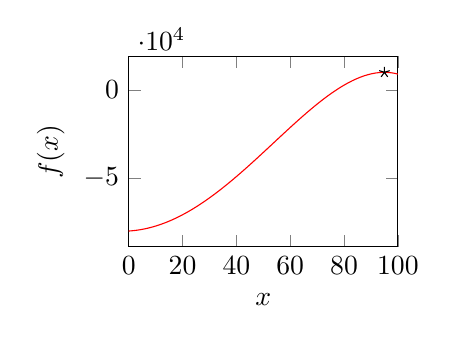
\begin{tikzpicture}
    \begin{axis}[
      height = {4cm},
      ylabel = {$f(x)$},
      xmin = {0},
      xmax = {100},
      xlabel = {$x$},
      width = {5cm}
    ]
    
    \addplot+[
      solid, red, mark=none
    ] coordinates {
      (0.0, -80250.0)
      (1.0, -80136.03600000001)
      (2.0, -79984.19600000001)
      (3.0, -79794.576)
      (4.0, -79567.296)
      (5.0, -79302.5)
      (6.0, -79000.356)
      (7.0, -78661.056)
      (8.0, -78284.816)
      (9.0, -77871.876)
      (10.0, -77422.5)
      (11.0, -76936.976)
      (12.0, -76415.61600000001)
      (13.0, -75858.75600000001)
      (14.0, -75266.756)
      (15.0, -74640.0)
      (16.0, -73978.89600000001)
      (17.0, -73283.876)
      (18.0, -72555.39600000001)
      (19.0, -71793.936)
      (20.0, -71000.0)
      (21.0, -70174.116)
      (22.0, -69316.836)
      (23.0, -68428.736)
      (24.0, -67510.41600000001)
      (25.0, -66562.5)
      (26.0, -65585.636)
      (27.0, -64580.496)
      (28.0, -63547.776)
      (29.0, -62488.195999999996)
      (30.0, -61402.5)
      (31.0, -60291.456000000006)
      (32.0, -59155.856)
      (33.0, -57996.516)
      (34.0, -56814.276)
      (35.0, -55610.0)
      (36.0, -54384.576)
      (37.0, -53138.916)
      (38.0, -51873.956000000006)
      (39.0, -50590.656)
      (40.0, -49290.0)
      (41.0, -47972.996)
      (42.0, -46640.67600000001)
      (43.0, -45294.096000000005)
      (44.0, -43934.336)
      (45.0, -42562.5)
      (46.0, -41179.71600000001)
      (47.0, -39787.136000000006)
      (48.0, -38385.936)
      (49.0, -36977.316)
      (50.0, -35562.5)
      (51.0, -34142.736)
      (52.0, -32719.296000000002)
      (53.0, -31293.476000000002)
      (54.0, -29866.595999999998)
      (55.0, -28440.0)
      (56.0, -27015.056000000004)
      (57.0, -25593.155999999995)
      (58.0, -24175.716)
      (59.0, -22764.176)
      (60.0, -21360.000000000004)
      (61.0, -19964.676)
      (62.0, -18579.716)
      (63.0, -17206.656)
      (64.0, -15847.056)
      (65.0, -14502.5)
      (66.0, -13174.595999999998)
      (67.0, -11864.976000000002)
      (68.0, -10575.295999999998)
      (69.0, -9307.236)
      (70.0, -8062.5)
      (71.0, -6842.8160000000025)
      (72.0, -5649.9360000000015)
      (73.0, -4485.636)
      (74.0, -3351.7160000000003)
      (75.0, -2250.0)
      (76.0, -1182.3359999999993)
      (77.0, -150.59599999999955)
      (78.0, 843.3240000000005)
      (79.0, 1797.503999999999)
      (80.0, 2710.0)
      (81.0, 3578.844)
      (82.0, 4402.044)
      (83.0, 5177.584)
      (84.0, 5903.424)
      (85.0, 6577.5)
      (86.0, 7197.724)
      (87.0, 7761.984)
      (88.0, 8268.144)
      (89.0, 8714.044)
      (90.0, 9097.5)
      (91.0, 9416.304)
      (92.0, 9668.224)
      (93.0, 9851.004)
      (94.0, 9962.364)
      (95.0, 10000.0)
      (96.0, 9961.584)
      (97.0, 9844.764)
      (98.0, 9647.164)
      (99.0, 9366.384)
      (100.0, 9000.0)
      (101.0, 8545.564)
      (102.0, 8000.603999999999)
      (103.0, 7362.624)
      (104.0, 6629.103999999999)
      (105.0, 5797.5)
      (106.0, 4865.244000000001)
      (107.0, 3829.7439999999997)
      (108.0, 2688.383999999999)
      (109.0, 1438.5239999999994)
      (110.0, 77.5)
      (111.0, -1397.3760000000002)
      (112.0, -2988.815999999999)
      (113.0, -4699.5560000000005)
      (114.0, -6532.356)
      (115.0, -8490.0)
      (116.0, -10575.295999999998)
      (117.0, -12791.076000000001)
      (118.0, -15140.196)
      (119.0, -17625.536000000004)
      (120.0, -20250.0)
    };
    
    \addplot+[
      draw = none,
      black, mark=star
    ] coordinates {
      (95.0, 10000.0)
    };
    
    \end{axis}
    \end{tikzpicture}
    
            
            \end{figure} 
            \item The optimal solution is $x^* = 95$.
            \item The value of the optimal solution is $f(x^*) = 10000$ (million Rupiah).   
        \end{itemize}
    \end{itemize}
\end{frame}


\begin{frame}{About the model and its optimal solution(s)}
    \begin{itemize}[<+->]
        \item We can have multiple optimal solutions.
        \begin{figure}
            \centering
            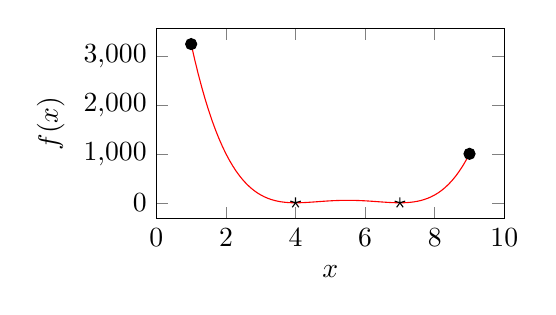
\begin{tikzpicture}[]
    \begin{axis}[
      height = {4cm},
      ylabel = {$f(x)$},
      xmin = {0},
      xmax = {10},
      xlabel = {$x$},
      width = {6cm}
    ]
    
    \addplot+[
      solid, red, mark=none
    ] coordinates {
      (1.0, 3240.0)
      (1.1, 2927.521)
      (1.2, 2637.3759999999997)
      (1.3, 2368.521)
      (1.4, 2119.936)
      (1.5, 1890.625)
      (1.6, 1679.616)
      (1.7, 1485.9609999999998)
      (1.8, 1308.7360000000003)
      (1.9, 1147.041)
      (2.0, 1000.0)
      (2.1, 866.7610000000002)
      (2.2, 746.4959999999998)
      (2.3, 638.4010000000002)
      (2.4, 541.696)
      (2.5, 455.625)
      (2.6, 379.456)
      (2.7, 312.4809999999999)
      (2.8, 254.01600000000008)
      (2.9, 203.401)
      (3.0, 160.0)
      (3.1, 123.20099999999996)
      (3.2, 92.41599999999995)
      (3.3, 67.08100000000005)
      (3.4, 46.65600000000001)
      (3.5, 30.625)
      (3.6, 18.495999999999988)
      (3.7, 9.800999999999988)
      (3.8, 4.096000000000008)
      (3.9, 0.9610000000000017)
      (4.0, 0.0)
      (4.1, 0.8409999999999942)
      (4.2, 3.136000000000005)
      (4.3, 6.560999999999994)
      (4.4, 10.816000000000015)
      (4.5, 15.625)
      (4.6, 20.735999999999983)
      (4.7, 25.92100000000001)
      (4.8, 30.97599999999999)
      (4.9, 35.72100000000002)
      (5.0, 40.0)
      (5.1, 43.68099999999999)
      (5.2, 46.656000000000006)
      (5.3, 48.840999999999994)
      (5.4, 50.17600000000001)
      (5.5, 50.625)
      (5.6, 50.176)
      (5.7, 48.840999999999994)
      (5.8, 46.656)
      (5.9, 43.68099999999998)
      (6.0, 40.0)
      (6.1, 35.72100000000001)
      (6.2, 30.97599999999999)
      (6.3, 25.92100000000001)
      (6.4, 20.735999999999983)
      (6.5, 15.625)
      (6.6, 10.816000000000015)
      (6.7, 6.560999999999993)
      (6.8, 3.136000000000005)
      (6.9, 0.8409999999999943)
      (7.0, 0.0)
      (7.1, 0.960999999999993)
      (7.2, 4.096000000000008)
      (7.3, 9.800999999999988)
      (7.4, 18.496000000000038)
      (7.5, 30.625)
      (7.6, 46.655999999999935)
      (7.7, 67.08100000000005)
      (7.8, 92.41599999999995)
      (7.9, 123.2010000000001)
      (8.0, 160.0)
      (8.1, 203.40099999999987)
      (8.2, 254.0159999999996)
      (8.3, 312.48100000000045)
      (8.4, 379.45600000000024)
      (8.5, 455.625)
      (8.6, 541.6959999999997)
      (8.7, 638.4009999999992)
      (8.8, 746.4960000000008)
      (8.9, 866.7610000000004)
      (9.0, 1000.0)
    };
    
    \addplot+[
      draw = none,
      black, mark=star
    ] coordinates {
      (4.0, 0.0)
    };
    
    \addplot+[
      draw = none,
      black, mark=star
    ] coordinates {
      (7.0, 0.0)
    };
    
    \addplot+[
      draw = none,
      black, mark=*
    ] coordinates {
      (1.0, 3240.0)
      (9.0, 1000.0)
    };
    
    \end{axis}
    \end{tikzpicture}
    
    ~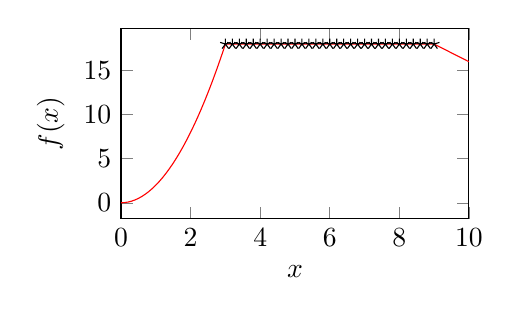
\begin{tikzpicture}[]
    \begin{axis}[
      height = {4cm},
      ylabel = {$f(x)$},
      xmin = {0},
      xmax = {10},
      xlabel = {$x$},
      width = {6cm}
    ]
    
    \addplot+[
      solid, red, mark=none
    ] coordinates {
      (0.0, 0.0)
      (0.1, 0.020000000000000004)
      (0.2, 0.08000000000000002)
      (0.3, 0.18)
      (0.4, 0.32000000000000006)
      (0.5, 0.5)
      (0.6, 0.72)
      (0.7, 0.9799999999999999)
      (0.8, 1.2800000000000002)
      (0.9, 1.62)
      (1.0, 2.0)
      (1.1, 2.4200000000000004)
      (1.2, 2.88)
      (1.3, 3.3800000000000003)
      (1.4, 3.9199999999999995)
      (1.5, 4.5)
      (1.6, 5.120000000000001)
      (1.7, 5.779999999999999)
      (1.8, 6.48)
      (1.9, 7.22)
      (2.0, 8.0)
      (2.1, 8.82)
      (2.2, 9.680000000000001)
      (2.3, 10.579999999999998)
      (2.4, 11.52)
      (2.5, 12.5)
      (2.6, 13.520000000000001)
      (2.7, 14.580000000000002)
      (2.8, 15.679999999999998)
      (2.9, 16.82)
      (3.0, 18.0)
      (3.1, 18)
      (3.2, 18)
      (3.3, 18)
      (3.4, 18)
      (3.5, 18)
      (3.6, 18)
      (3.7, 18)
      (3.8, 18)
      (3.9, 18)
      (4.0, 18)
      (4.1, 18)
      (4.2, 18)
      (4.3, 18)
      (4.4, 18)
      (4.5, 18)
      (4.6, 18)
      (4.7, 18)
      (4.8, 18)
      (4.9, 18)
      (5.0, 18)
      (5.1, 18)
      (5.2, 18)
      (5.3, 18)
      (5.4, 18)
      (5.5, 18)
      (5.6, 18)
      (5.7, 18)
      (5.8, 18)
      (5.9, 18)
      (6.0, 18)
      (6.1, 18)
      (6.2, 18)
      (6.3, 18)
      (6.4, 18)
      (6.5, 18)
      (6.6, 18)
      (6.7, 18)
      (6.8, 18)
      (6.9, 18)
      (7.0, 18)
      (7.1, 18)
      (7.2, 18)
      (7.3, 18)
      (7.4, 18)
      (7.5, 18)
      (7.6, 18)
      (7.7, 18)
      (7.8, 18)
      (7.9, 18)
      (8.0, 18)
      (8.1, 18)
      (8.2, 18)
      (8.3, 18)
      (8.4, 18)
      (8.5, 18)
      (8.6, 18)
      (8.7, 18)
      (8.8, 18)
      (8.9, 18)
      (9.0, 18)
      (9.1, 17.8)
      (9.2, 17.6)
      (9.3, 17.4)
      (9.4, 17.2)
      (9.5, 17.0)
      (9.6, 16.8)
      (9.7, 16.6)
      (9.8, 16.4)
      (9.9, 16.2)
      (10.0, 16.0)
    };
    
    \addplot+[
      draw = none,
      black, mark=star
    ] coordinates {
      (3.0, 18.0)
      (3.2, 18)
      (3.4, 18)
      (3.6, 18)
      (3.8, 18)
      (4.0, 18)
      (4.2, 18)
      (4.4, 18)
      (4.6, 18)
      (4.8, 18)
      (5.0, 18)
      (5.2, 18)
      (5.4, 18)
      (5.6, 18)
      (5.8, 18)
      (6.0, 18)
      (6.2, 18)
      (6.4, 18)
      (6.6, 18)
      (6.8, 18)
      (7.0, 18)
      (7.2, 18)
      (7.4, 18)
      (7.6, 18)
      (7.8, 18)
      (8.0, 18)
      (8.2, 18)
      (8.4, 18)
      (8.6, 18)
      (8.8, 18)
      (9.0, 18)
    };
    
    \end{axis}
    \end{tikzpicture}
    
            
        \end{figure} 
    \end{itemize}        
\end{frame}


\begin{frame}{About the model and its optimal solution(s)}
    \begin{itemize}[<+->]
        \item The decision variable can be multi-dimensional.
        \begin{equation}
            \begin{aligned}
                & \underset{x_1, x_2}{\text{minimize}}
                & & (x_1-2)^2 \cdot (x_2-3)^2 \cdot \left(x_1 x_2 - \frac52 \right)\\
                & \text{subject to}
                & & 1 \leq x_1 \leq 4, \\
                & & & 1 \leq x_2 \leq 4.
            \end{aligned}
            \label{eq:2D_optimization}
        \end{equation}
        \begin{figure}
            \centering
            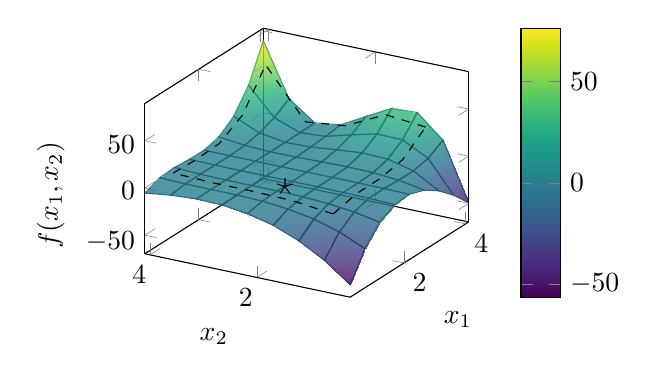
\begin{tikzpicture}
    \begin{axis}[
        view={-60}{30},
        grid=minor,
        colormap/viridis,
        xlabel={$x_1$},
        ylabel={$x_2$},
        zlabel={$f(x_1, x_2)$},
        scale=0.6,
        colorbar,
        domain=0.25:4.1,
        y domain=0.25:4.1,
        samples=9
    ]
        \addplot3[
            surf,
            opacity=0.8,
            shader=faceted interp,
        ] {(x-2)^2*(y-3)^2*(x*y-2.5)};

        %add plot at the optimal solution
        \addplot3[
            mark=star,
            mark size=3,
            only marks,
            mark options={draw=black},
        ] coordinates {(1.438, 2.158, 0.1350)};

        %add lines for the feasible region at function height with intermediate points
        \addplot3[
            mark=none,
            style=dashed,
            color=black,
        ] coordinates {
            (1, 1, {(1-2)^2*(1-3)^2*(1*1-2.5)}) 
            (1.75, 1, {(1.75-2)^2*(1-3)^2*(1.75*1-2.5)})
            (2.5, 1, {(2.5-2)^2*(1-3)^2*(2.5*1-2.5)})
            (3.25, 1, {(3.25-2)^2*(1-3)^2*(3.25*1-2.5)})
            (4, 1, {(4-2)^2*(1-3)^2*(4*1-2.5)})
        };

        \addplot3[
            mark=none,
            style=dashed,
            color=black,
        ] coordinates {
            (1, 4, {(1-2)^2*(4-3)^2*(1*4-2.5)}) 
            (1.75, 4, {(1.75-2)^2*(4-3)^2*(1.75*4-2.5)})
            (2.5, 4, {(2.5-2)^2*(4-3)^2*(2.5*4-2.5)})
            (3.25, 4, {(3.25-2)^2*(4-3)^2*(3.25*4-2.5)})
            (4, 4, {(4-2)^2*(4-3)^2*(4*4-2.5)})
        };

        \addplot3[
            mark=none,
            style=dashed,
            color=black,
        ] coordinates {
            (1, 1, {(1-2)^2*(1-3)^2*(1*1-2.5)}) 
            (1, 1.75, {(1-2)^2*(1.75-3)^2*(1*1.75-2.5)})
            (1, 2.5, {(1-2)^2*(2.5-3)^2*(1*2.5-2.5)})
            (1, 3.25, {(1-2)^2*(3.25-3)^2*(1*3.25-2.5)})
            (1, 4, {(1-2)^2*(4-3)^2*(1*4-2.5)})
        };

        \addplot3[
            mark=none,
            style=dashed,
            color=black,
        ] coordinates {
            (4, 1, {(4-2)^2*(1-3)^2*(4*1-2.5)}) 
            (4, 1.75, {(4-2)^2*(1.75-3)^2*(4*1.75-2.5)})
            (4, 2.5, {(4-2)^2*(2.5-3)^2*(4*2.5-2.5)})
            (4, 3.25, {(4-2)^2*(3.25-3)^2*(4*3.25-2.5)})
            (4, 4, {(4-2)^2*(4-3)^2*(4*4-2.5)})
        };
        
    \end{axis}
\end{tikzpicture}
        \end{figure}
        \item $x_1^* = 1.438$, $x_2^* = 2.158$, $f(x_1^*, x_2^*) = 0.1350$.
    \end{itemize}
\end{frame}


\begin{frame}{About the model and its optimal solution(s)}
    \begin{itemize}[<+->]
        \item The decision variable can be multi-dimensional.
        \begin{figure}
            \centering
            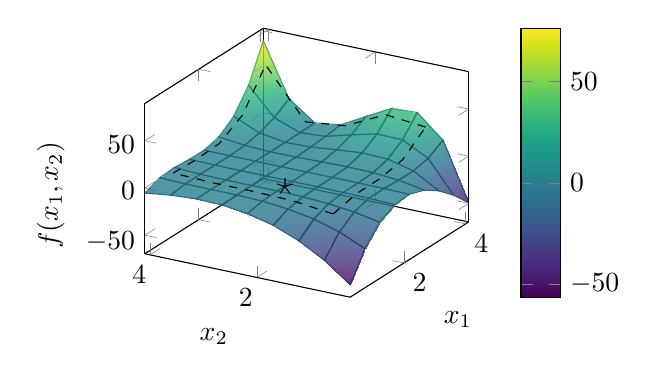
\begin{tikzpicture}
    \begin{axis}[
        view={-60}{30},
        grid=minor,
        colormap/viridis,
        xlabel={$x_1$},
        ylabel={$x_2$},
        zlabel={$f(x_1, x_2)$},
        scale=0.6,
        colorbar,
        domain=0.25:4.1,
        y domain=0.25:4.1,
        samples=9
    ]
        \addplot3[
            surf,
            opacity=0.8,
            shader=faceted interp,
        ] {(x-2)^2*(y-3)^2*(x*y-2.5)};

        %add plot at the optimal solution
        \addplot3[
            mark=star,
            mark size=3,
            only marks,
            mark options={draw=black},
        ] coordinates {(1.438, 2.158, 0.1350)};

        %add lines for the feasible region at function height with intermediate points
        \addplot3[
            mark=none,
            style=dashed,
            color=black,
        ] coordinates {
            (1, 1, {(1-2)^2*(1-3)^2*(1*1-2.5)}) 
            (1.75, 1, {(1.75-2)^2*(1-3)^2*(1.75*1-2.5)})
            (2.5, 1, {(2.5-2)^2*(1-3)^2*(2.5*1-2.5)})
            (3.25, 1, {(3.25-2)^2*(1-3)^2*(3.25*1-2.5)})
            (4, 1, {(4-2)^2*(1-3)^2*(4*1-2.5)})
        };

        \addplot3[
            mark=none,
            style=dashed,
            color=black,
        ] coordinates {
            (1, 4, {(1-2)^2*(4-3)^2*(1*4-2.5)}) 
            (1.75, 4, {(1.75-2)^2*(4-3)^2*(1.75*4-2.5)})
            (2.5, 4, {(2.5-2)^2*(4-3)^2*(2.5*4-2.5)})
            (3.25, 4, {(3.25-2)^2*(4-3)^2*(3.25*4-2.5)})
            (4, 4, {(4-2)^2*(4-3)^2*(4*4-2.5)})
        };

        \addplot3[
            mark=none,
            style=dashed,
            color=black,
        ] coordinates {
            (1, 1, {(1-2)^2*(1-3)^2*(1*1-2.5)}) 
            (1, 1.75, {(1-2)^2*(1.75-3)^2*(1*1.75-2.5)})
            (1, 2.5, {(1-2)^2*(2.5-3)^2*(1*2.5-2.5)})
            (1, 3.25, {(1-2)^2*(3.25-3)^2*(1*3.25-2.5)})
            (1, 4, {(1-2)^2*(4-3)^2*(1*4-2.5)})
        };

        \addplot3[
            mark=none,
            style=dashed,
            color=black,
        ] coordinates {
            (4, 1, {(4-2)^2*(1-3)^2*(4*1-2.5)}) 
            (4, 1.75, {(4-2)^2*(1.75-3)^2*(4*1.75-2.5)})
            (4, 2.5, {(4-2)^2*(2.5-3)^2*(4*2.5-2.5)})
            (4, 3.25, {(4-2)^2*(3.25-3)^2*(4*3.25-2.5)})
            (4, 4, {(4-2)^2*(4-3)^2*(4*4-2.5)})
        };
        
    \end{axis}
\end{tikzpicture}
        \end{figure}
        \item There are values in the plot with lower objective values than the optimal solution. Why are they not optimal?
    \end{itemize}
\end{frame}


\begin{frame}{Sometimes the objective function itself is not fully known}
    \begin{itemize}[<+->]
        \item Example [Exercise 2.3]:
        \begin{equation}
            \begin{aligned}
                & \underset{x}{\text{maximize}}
                & & f(x) = \text{CO}_2 \text{ capture economic value}(x) - x \\
                & \text{subject to}
                & & 0 \leq x \leq 1 \text{ billion Rupiah}.
            \end{aligned}
            \label{eq:Qertamina_optimization}
        \end{equation}
        \item $f(x)$ is only evaluated at $x \in \{0, 100, 200, \ldots, 1000\}$ million Rupiah. 
        \begin{figure}
            \centering
            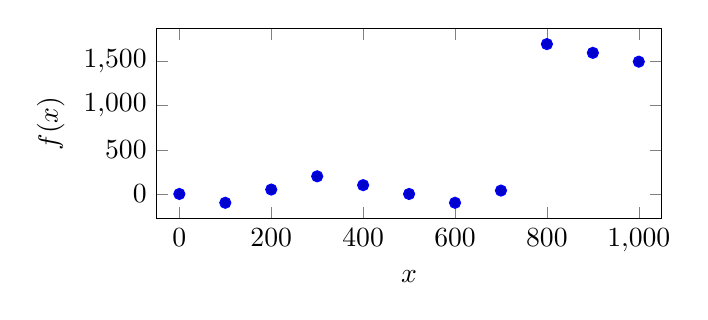
\begin{tikzpicture}[]
    \begin{axis}[
      height = {4cm},
      ylabel = {$f(x)$},
      xmin = {-50},
      xmax = {1050},
      xlabel = {$x$},
      width = {8cm}
    ]
    
    \addplot+[
      draw = none,
      mark=*
    ] coordinates {
      (0.0, 1.0305768090951019e-6)
      (100.0, -99.97730106564879)
      (200.0, 50.0)
      (300.0, 199.97730106564876)
      (400.0, 99.99999896944848)
      (500.0, 5.578468744715792e-7)
      (600.0, -99.98771165079557)
      (700.0, 38.405844044235096)
      (800.0, 1699.3292997390672)
      (900.0, 1599.999969540041)
      (1000.0, 1499.999999998617)
    };
    
    \end{axis}
    \end{tikzpicture}
    
    
        \end{figure}
        \item What is the optimal solution? If you are given more chances to evaluate $f(x)$ at some $x$'s, which $x$ values would you choose?
        
    \end{itemize}
\end{frame}

\begin{frame}{Summary}
    \begin{itemize}[<+->]
        \item When modeling an optimization problem, spend time to identify the objective function, decision variables, constraints, and parameters (and therefore the data you need).
        \item The optimal solution is the value of the decision variable that minimizes (or maximizes) the objective function.
        \item The optimal solution can be multi-dimensional, and there can be multiple optimal solutions.
    \end{itemize}
\end{frame}

\section{Examples}
\begin{frame}{Let's now take a look at some examples}
    \begin{itemize}[<+->]
        \item Example 1: \href{https://colab.research.google.com/drive/1fkSbxvqUKUXSYWVWAXwGBWoc-8NCRFHS?usp=sharing}{PLX profit maximization}
        \item Example 2: \href{https://colab.research.google.com/drive/1dvgO3HJ0mT7kNphkEqfGdHYISbJ2lT_r?usp=sharing}{2D optimization problem}
        \item Example 3: \href{https://colab.research.google.com/drive/1wPqfn7aTNdO3aikmQnaeyLAeLD4yh4VK?usp=sharing}{Production planning}
    \end{itemize}
\end{frame}


\begin{frame}{What's next?}
    \begin{itemize}[<+->]
        \item Next week: 
        \begin{itemize}[<+->]
            \item Data Collection and Processing (Ch. 3)
            \item Proposal Presentation (Group 1-2, random order)
        \end{itemize}
        \item Next reading: Ch. 3 -- Data Collection and Processing
    \end{itemize}
\end{frame}

\begin{frame}{Thank you!}
    \begin{itemize}[<+->]
        \item Questions?
    \end{itemize}
\end{frame}











\end{document}
